\documentclass[12pt]{article}

% Packages
\usepackage[margin=2.5cm]{geometry}
\usepackage{amsmath}
\usepackage{amssymb}
\usepackage{bm}
\usepackage{graphicx}
\usepackage{physics}
\usepackage{tikz}
\usetikzlibrary{arrows.meta, positioning, shapes.geometric,
	decorations.pathmorphing, calc, fit, backgrounds}
\usepackage{float}
\usepackage{booktabs}
\usepackage{multirow}
\usepackage{array}
\usepackage{longtable}
\usepackage{xcolor}
\usepackage{hyperref}

% Better boxes
\usepackage{amsfonts}

% No indentation
\setlength{\parindent}{0pt}
\setlength{\parskip}{6pt}

% Custom colours for workflow diagram
\definecolor{step1}{HTML}{E8F5E9}
\definecolor{step2}{HTML}{E3F2FD}
\definecolor{step3}{HTML}{FFF3E0}
\definecolor{step4}{HTML}{F3E5F5}
\definecolor{step5}{HTML}{FFEBEE}
\definecolor{step6}{HTML}{E0F7FA}
\definecolor{step7}{HTML}{FFF9C4}
\definecolor{stepborder}{HTML}{455A64}

\begin{document}

\title{Guidelines for Adsorption Isotherm Analysis:\\
	Workflow, Energy Distributions, and Statistical Comparison}
\author{}
\date{February 16, 2026}
\maketitle

\tableofcontents
\newpage

% =====================================================================
%  SECTION 1: WORKFLOW
% =====================================================================
\section{Complete analysis workflow}
\label{sec:workflow}

The analysis of adsorption equilibrium data follows a structured
seven-step workflow.  Each step builds on the previous one, culminating
in a set of model-independent descriptors that enable cross-system
comparison and material classification.

\subsection{Overview}

Figure~\ref{fig:workflow} presents the complete workflow as a
sequential pipeline.  The steps are:

\begin{enumerate}
	\item \textbf{Experimental measurements}: collect equilibrium
	pairs $(C_{e,i},\, q_{e,i})$ under controlled conditions.
	\item \textbf{Isotherm fitting}: fit all candidate isotherm models
	by non-linear least-squares regression.
	\item \textbf{Error metrics}: compute residual error metrics
	(SSE, $R^2$, ARED, HYBRID, MPSED) and information criteria
	(AIC$_c$, BIC).
	\item \textbf{Model selection}: choose the best model using AIC/BIC
	ranking, F-tests for nested models, and residual analysis.
	\item \textbf{Report $E_{\mathrm{ads}}$ and $f(E)$}: extract the
	universal descriptors $\{Q_{\max},\, K_{\mathrm{aff}}^{\ast},\,
	E_{\mathrm{aff}},\, \sigma_E\}$ and the energy distribution.
	\item \textbf{Statistical tests}: compare materials using
	energy-distribution overlap, F-tests, and Akaike weights.
	\item \textbf{Clustering}: group materials by similarity in
	descriptor space using KNN, SVM, or hierarchical clustering.
\end{enumerate}

\begin{figure}[H]
	\centering
	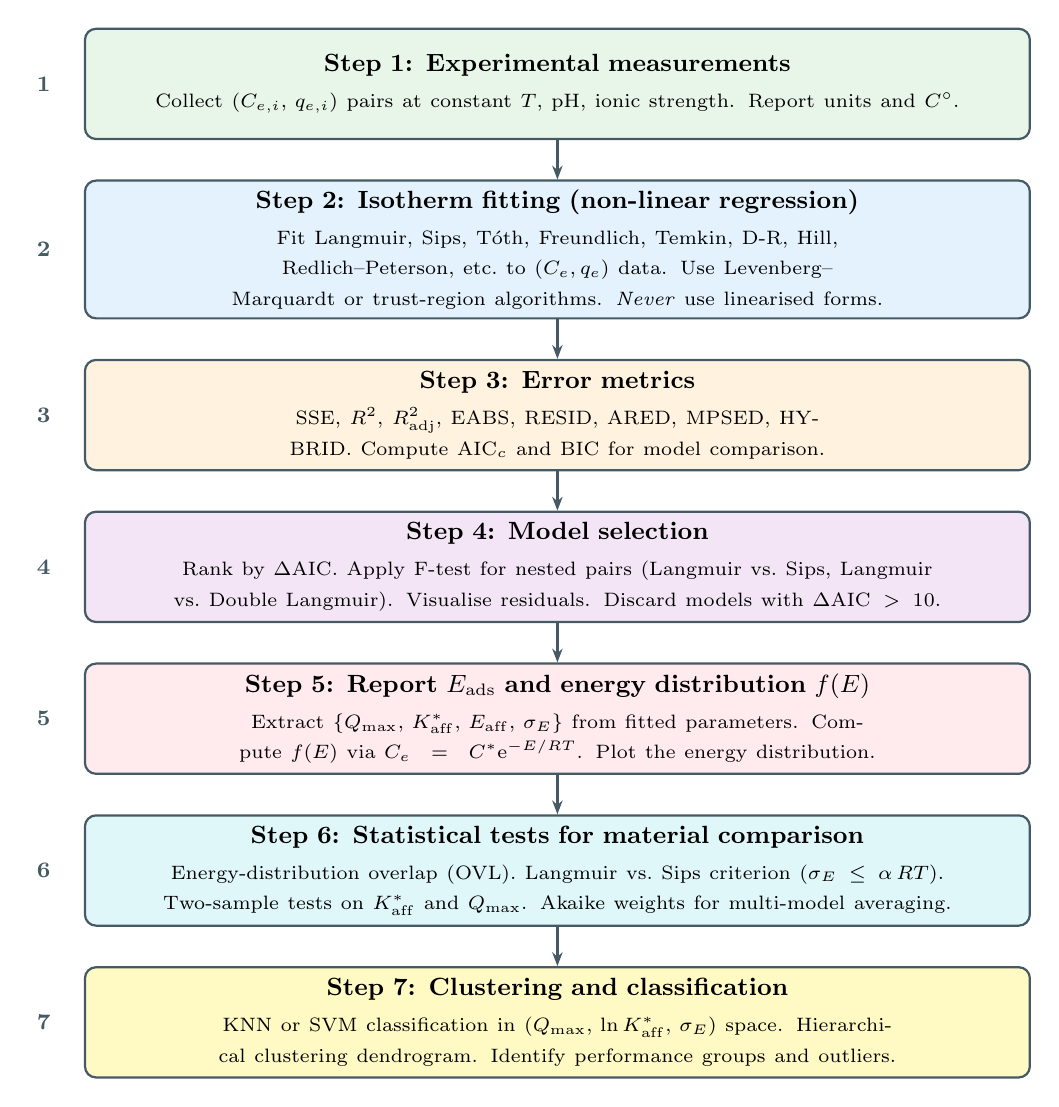
\begin{tikzpicture}[
		every node/.style={font=\small},
		stepbox/.style={draw=stepborder, rounded corners=4pt,
			minimum width=12cm, minimum height=1.4cm,
			align=center, thick, text width=11cm},
		arr/.style={-{Stealth[length=5pt]}, thick, stepborder},
		lbl/.style={font=\footnotesize\bfseries, stepborder},
		detail/.style={font=\scriptsize, text width=10.5cm, align=left},
		]
		% Step 1
		\node[stepbox, fill=step1] (s1)
		{\textbf{Step 1: Experimental measurements}\\[2pt]
			{\scriptsize Collect $(C_{e,i},\, q_{e,i})$ pairs at constant $T$,
				$\text{pH}$, ionic strength.  Report units and $C^\circ$.}};

		% Step 2
		\node[stepbox, fill=step2, below=0.5cm of s1] (s2)
		{\textbf{Step 2: Isotherm fitting (non-linear regression)}\\[2pt]
			{\scriptsize Fit Langmuir, Sips, T\'{o}th, Freundlich, Temkin,
				D-R, Hill, Redlich--Peterson, etc.\ to $(C_e, q_e)$ data.
				Use Levenberg--Marquardt or trust-region algorithms.
				\emph{Never} use linearised forms.}};

		% Step 3
		\node[stepbox, fill=step3, below=0.5cm of s2] (s3)
		{\textbf{Step 3: Error metrics}\\[2pt]
			{\scriptsize SSE, $R^2$, $R^2_{\mathrm{adj}}$, EABS, RESID,
				ARED, MPSED, HYBRID.  Compute AIC$_c$ and BIC for
				model comparison.}};

		% Step 4
		\node[stepbox, fill=step4, below=0.5cm of s3] (s4)
		{\textbf{Step 4: Model selection}\\[2pt]
			{\scriptsize Rank by $\Delta$AIC.  Apply F-test for nested pairs
				(Langmuir vs.\ Sips, Langmuir vs.\ Double Langmuir).
				Visualise residuals.  Discard models with
				$\Delta\mathrm{AIC} > 10$.}};

		% Step 5
		\node[stepbox, fill=step5, below=0.5cm of s4] (s5)
		{\textbf{Step 5: Report $E_{\mathrm{ads}}$ and energy
				distribution $f(E)$}\\[2pt]
			{\scriptsize Extract $\{Q_{\max},\, K_{\mathrm{aff}}^{\ast},\,
				E_{\mathrm{aff}},\, \sigma_E\}$ from fitted parameters.
				Compute $f(E)$ via $C_e = C^{\ast}\mathrm{e}^{-E/RT}$.
				Plot the energy distribution.}};

		% Step 6
		\node[stepbox, fill=step6, below=0.5cm of s5] (s6)
		{\textbf{Step 6: Statistical tests for material comparison}\\[2pt]
			{\scriptsize Energy-distribution overlap (OVL).  Langmuir vs.\ Sips
				criterion ($\sigma_E \leq \alpha\,RT$).
				Two-sample tests on $K_{\mathrm{aff}}^{\ast}$ and $Q_{\max}$.
				Akaike weights for multi-model averaging.}};

		% Step 7
		\node[stepbox, fill=step7, below=0.5cm of s6] (s7)
		{\textbf{Step 7: Clustering and classification}\\[2pt]
			{\scriptsize KNN or SVM classification in
				$(Q_{\max},\, \ln K_{\mathrm{aff}}^{\ast},\, \sigma_E)$ space.
				Hierarchical clustering dendrogram.
				Identify performance groups and outliers.}};

		% Arrows
		\draw[arr] (s1) -- (s2);
		\draw[arr] (s2) -- (s3);
		\draw[arr] (s3) -- (s4);
		\draw[arr] (s4) -- (s5);
		\draw[arr] (s5) -- (s6);
		\draw[arr] (s6) -- (s7);

		% Step numbers
		\foreach \i/\c in {1/s1, 2/s2, 3/s3, 4/s4, 5/s5, 6/s6, 7/s7} {
			\node[lbl, anchor=east] at ([xshift=-0.3cm]\c.west) {\i};
		}
	\end{tikzpicture}
	\caption{Complete analysis workflow: from experimental measurements
		to material classification.  Each step builds on the previous one.
		Steps~1--4 are model-dependent; Steps~5--7 yield model-independent
		descriptors and statistical comparisons.}
	\label{fig:workflow}
\end{figure}

% =====================================================================
%  SECTION 1.1: Step 1 -- Measurements
% =====================================================================
\subsection{Step 1: Experimental measurements}

Adsorption equilibrium data are collected as pairs
$(C_{e,i},\, q_{e,i})$ at constant temperature $T$, pH, and ionic
strength.  The following information must be reported:

\begin{itemize}
	\item Concentration units for $C_e$ (e.g.\ mg\,L$^{-1}$,
	mmol\,L$^{-1}$).
	\item Capacity units for $q_e$ (e.g.\ mg\,g$^{-1}$,
	mmol\,g$^{-1}$).
	\item The standard-state concentration $C^\circ$ chosen for
	thermodynamic analysis (e.g.\ $1$~mg\,L$^{-1}$ or
	$1$~mol\,L$^{-1}$).
	\item Temperature, pH, and contact time.
	\item Number of data points $n$ and replicate information.
\end{itemize}

% =====================================================================
%  SECTION 1.2: Step 2 -- Fitting
% =====================================================================
\subsection{Step 2: Isotherm fitting}

All candidate models should be fitted simultaneously to the same
dataset by non-linear least-squares regression:
\begin{equation}
	\min_{\boldsymbol{\theta}}\;
	\sum_{i=1}^{n}
	\bigl(q_{e,i}^{\exp} - q(C_{e,i};\,\boldsymbol{\theta})\bigr)^{2},
\end{equation}
where $\boldsymbol{\theta}$ is the parameter vector of each model.

\paragraph{Implementation notes.}
\begin{itemize}
	\item Use Levenberg--Marquardt or trust-region-reflective
	algorithms.
	\item Provide physically meaningful initial guesses:
	$Q_{\max} \approx \max(q_e)$, $K_L \approx 1/C_{e,\text{mid}}$.
	\item Impose bound constraints: $Q_{\max} > 0$, $K > 0$,
	$0 < n \leq 1$ (or $n > 0$ for general heterogeneity).
	\item \textbf{Never} use linearised forms ($1/q_e$ vs.\
	$1/C_e$) because they distort the error structure.
\end{itemize}

Table~\ref{tab:models_summary} lists the candidate models with
their number of parameters.

\begin{table}[H]
	\centering
	\small
	\caption{Candidate isotherm models and their number of free
		parameters~$p$.}
	\label{tab:models_summary}
	\renewcommand{\arraystretch}{1.3}
	\begin{tabular}{llcc}
		\toprule
		\textbf{Model} & \textbf{Equation} & $\boldsymbol{p}$
		& \textbf{Nested in} \\
		\midrule
		Henry
		& $q_e = K_H C_e$
		& 1 & Langmuir \\
		Langmuir
		& $q_e = Q_{\max} K_L C_e/(1 + K_L C_e)$
		& 2 & Sips, T\'{o}th, Double L. \\
		Double Langmuir
		& $q_e = \sum_{i=1}^{2} Q_i K_i C_e/(1 + K_i C_e)$
		& 4 & --- \\
		Freundlich
		& $q_e = K_F C_e^{1/n}$
		& 2 & --- \\
		Sips (L--F)
		& $q_e = Q_{\max}(K_S C_e)^m/[1+(K_S C_e)^m]$
		& 3 & --- \\
		T\'{o}th
		& $q_e = q_{\max} b C_e/[1+(bC_e)^t]^{1/t}$
		& 3 & --- \\
		Jovanovic
		& $q_e = q_{\max}[1-\exp(-bC_e)]$
		& 2 & --- \\
		Temkin
		& $q_e = (RT/b_T)\ln(a_T C_e)$
		& 2 & --- \\
		UNILAN
		& $q_e = (q_{\max}/2s)\ln[(1+b_{\max}C_e)/(1+b_{\min}C_e)]$
		& 3 & --- \\
		Redlich--Peterson
		& $q_e = K_{RP}C_e/(1 + a_{RP}C_e^{\beta})$
		& 3 & Langmuir \\
		D-R
		& $q_e = Q_{\max}\exp[-(\varepsilon/E_a)^2]$
		& 2 & D-A \\
		D-A
		& $q_e = Q_{\max}\exp[-(\varepsilon/E_a)^{n_{DA}}]$
		& 3 & --- \\
		Hill
		& $q_e = Q_{\max}C_e^{n_H}/(K_D + C_e^{n_H})$
		& 3 & --- \\
		\bottomrule
	\end{tabular}
\end{table}

% =====================================================================
%  SECTION 1.3: Step 3 -- Error metrics
% =====================================================================
\subsection{Step 3: Error metrics}

After fitting, compute the following metrics for each model.

\subsubsection{Residual error metrics}

\begin{align}
	\text{SSE}   &= \sum_{i=1}^{n}(q_i^{\exp} - q_i^{\mathrm{pred}})^2,
	\label{eq:SSE} \\[4pt]
	R^2          &= 1 - \frac{\mathrm{SSE}}{\mathrm{SST}},
	\qquad \mathrm{SST} = \sum_{i}(q_i^{\exp} - \bar{q})^2,
	\label{eq:R2} \\[4pt]
	R^2_{\mathrm{adj}} &= 1 - \frac{n-1}{n-p-1}(1-R^2),
	\label{eq:R2adj} \\[4pt]
	\text{EABS}  &= \sum_{i}|q_i^{\exp} - q_i^{\mathrm{pred}}|,
	\label{eq:EABS} \\[4pt]
	\text{RESID} &= \frac{1}{n}\sum_{i}|q_i^{\exp} - q_i^{\mathrm{pred}}|,
	\label{eq:RESID} \\[4pt]
	\text{ARED}  &= \frac{100}{n}\sum_{i}
	\left|\frac{q_i^{\exp} - q_i^{\mathrm{pred}}}{q_i^{\exp}}\right|,
	\label{eq:ARED} \\[4pt]
	\text{MPSED} &= 100 \times \mathrm{median}\!\left[
	\left(\frac{q_i^{\exp} - q_i^{\mathrm{pred}}}{q_i^{\exp}}\right)^{\!2}
	\right],
	\label{eq:MPSED} \\[4pt]
	\text{HYBRID} &= \frac{100}{n-p}\sum_{i}
	\frac{(q_i^{\exp} - q_i^{\mathrm{pred}})^2}{q_i^{\exp}}.
	\label{eq:HYBRID}
\end{align}

\subsubsection{Information criteria for model selection}

\begin{align}
	\text{AIC}   &= n\ln\!\left(\frac{\mathrm{SSE}}{n}\right) + 2p,
	\label{eq:AIC} \\[4pt]
	\text{AIC}_c &= \text{AIC} + \frac{2p(p+1)}{n-p-1},
	\label{eq:AICc} \\[4pt]
	\text{BIC}   &= n\ln\!\left(\frac{\mathrm{SSE}}{n}\right) + p\ln n.
	\label{eq:BIC}
\end{align}

The model with the \emph{lowest} AIC$_c$ (or BIC) is preferred.
$\Delta\mathrm{AIC} < 2$: substantial support;
$4 < \Delta\mathrm{AIC} < 7$: considerably less;
$\Delta\mathrm{AIC} > 10$: essentially no support.

% =====================================================================
%  SECTION 1.4: Step 4 -- Model selection
% =====================================================================
\subsection{Step 4: Model selection}

\subsubsection{Ranking procedure}
\begin{enumerate}
	\item Compute AIC$_c$ for all models; rank by $\Delta$AIC.
	\item For nested pairs (Langmuir $\subset$ Sips, Langmuir
	$\subset$ Double Langmuir, Langmuir $\subset$ Redlich--Peterson),
	apply the F-test:
	\begin{equation}
		F = \frac{(\mathrm{SSE}_1 - \mathrm{SSE}_2)/(p_2 - p_1)}
		{\mathrm{SSE}_2/(n - p_2)}.
		\label{eq:Ftest}
	\end{equation}
	\item Inspect residual plots for systematic patterns.
	\item Compute Akaike weights:
	\begin{equation}
		w_i = \frac{\exp(-\Delta\mathrm{AIC}_i/2)}
		{\sum_{j}\exp(-\Delta\mathrm{AIC}_j/2)}.
		\label{eq:Akaike_weight}
	\end{equation}
	\item If multiple models have $\Delta\mathrm{AIC} < 2$,
	report all and consider model averaging.
\end{enumerate}

\subsubsection{Decision tree}

The model-selection decision tree proceeds in three phases:
(i)~physical screening of the data shape,
(ii)~AIC ranking among applicable models, and
(iii)~nested-model tests with physical validation.
Figure~\ref{fig:decision_tree} gives the complete flowchart.

\begin{figure}[p]
	\centering
	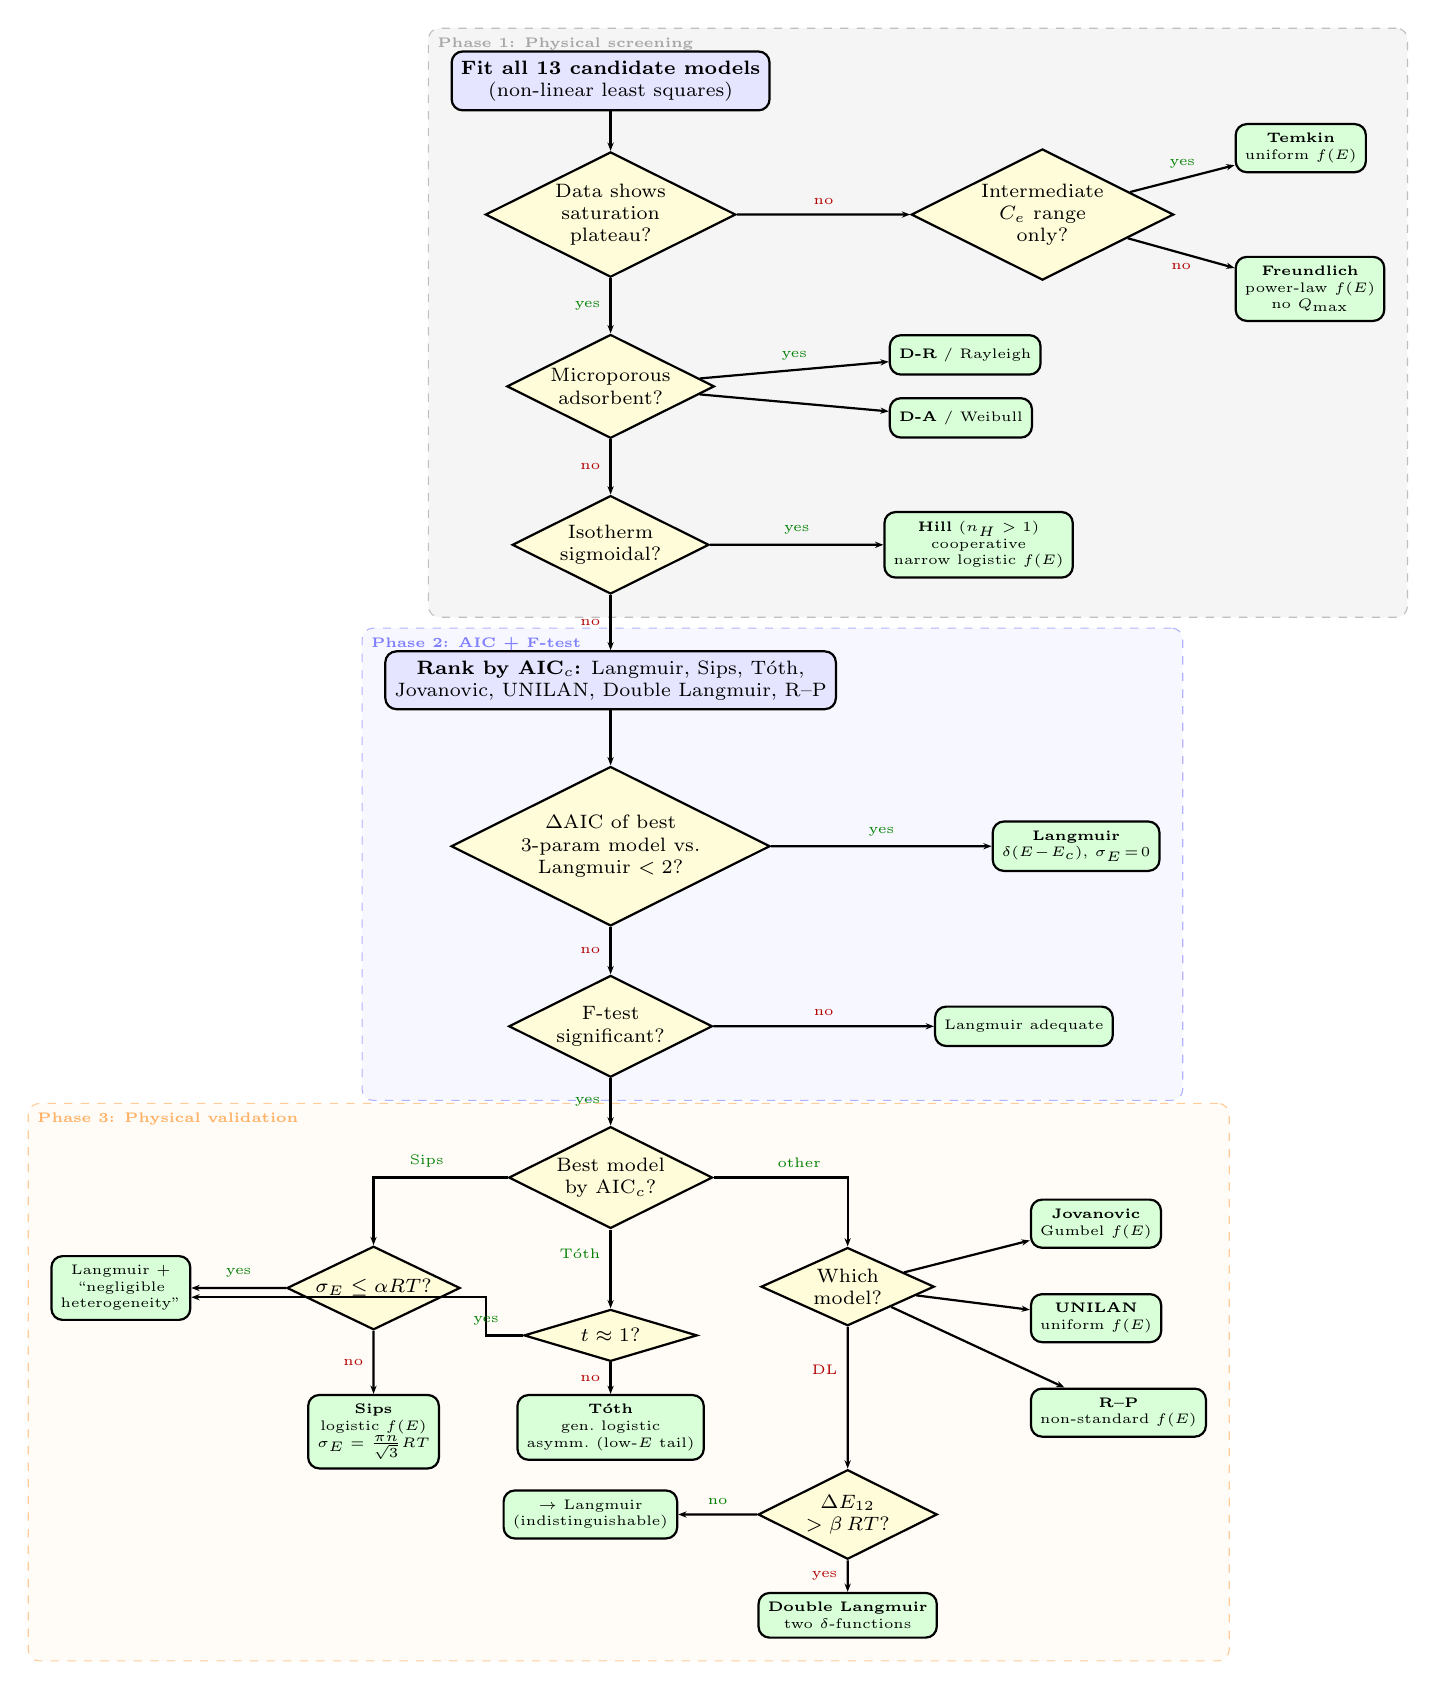
\begin{tikzpicture}[
		scale=0.78, every node/.append style={transform shape},
		every node/.style={font=\scriptsize},
		decision/.style={draw, diamond, aspect=2, inner sep=1pt,
			minimum width=2.2cm, align=center, thick, fill=yellow!15},
		result/.style={draw, rounded corners, minimum width=1.6cm,
			minimum height=0.5cm, align=center, thick, fill=green!15,
			font=\tiny},
		process/.style={draw, rounded corners, minimum width=2.2cm,
			minimum height=0.5cm, align=center, thick, fill=blue!10},
		arr/.style={-{Stealth[length=3pt]}, thick},
		yeslbl/.style={font=\tiny, green!50!black},
		nolbl/.style={font=\tiny, red!70!black},
		]

		% ============ PHASE 1: Physical screening ============
		\node[process] (fit) {\textbf{Fit all 13 candidate models}\\
			(non-linear least squares)};

		% --- Q1: saturation ---
		\node[decision, below=0.5cm of fit] (q1)
		{Data shows\\saturation\\plateau?};

		% NO saturation branch (right)
		\node[decision, right=2.2cm of q1] (q1b)
		{Intermediate\\$C_e$ range\\only?};
		\node[result, above right=0.1cm and 1.6cm of q1b] (r_temkin)
		{\textbf{Temkin}\\uniform $f(E)$};
		\node[result, below right=0.1cm and 1.6cm of q1b] (r_freund)
		{\textbf{Freundlich}\\power-law $f(E)$\\no $Q_{\max}$};

		% YES saturation branch (down)
		\node[decision, below=0.7cm of q1] (q2)
		{Microporous\\adsorbent?};

		% DR/DA branch (right)
		\node[result, right=2.2cm of q2, yshift=0.4cm] (r_DR)
		{\textbf{D-R} / Rayleigh};
		\node[result, right=2.2cm of q2, yshift=-0.4cm] (r_DA)
		{\textbf{D-A} / Weibull};

		% Continue down
		\node[decision, below=0.7cm of q2] (q3)
		{Isotherm\\sigmoidal?};

		% Hill branch (right)
		\node[result, right=2.2cm of q3] (r_hill)
		{\textbf{Hill} ($n_H > 1$)\\cooperative\\narrow logistic $f(E)$};

		% AIC ranking
		\node[process, below=0.7cm of q3] (aic)
		{\textbf{Rank by AIC$_c$:} Langmuir, Sips, T\'{o}th,\\
			Jovanovic, UNILAN, Double Langmuir, R--P};

		% ============ PHASE 2: AIC + F-test ============
		\node[decision, below=0.7cm of aic] (d1)
		{$\Delta\mathrm{AIC}$ of best\\3-param model vs.\\ Langmuir $< 2$?};
		\node[result, right=2.8cm of d1] (r_lang)
		{\textbf{Langmuir}\\$\delta(E\!-\!E_c)$, $\sigma_E\!=\!0$};

		\node[decision, below=0.6cm of d1] (d2)
		{F-test\\significant?};
		\node[result, right=2.8cm of d2] (r_lang2)
		{Langmuir adequate};

		% ============ PHASE 3: Which heterogeneous model? ============
		\node[decision, below=0.6cm of d2] (d3)
		{Best model\\by AIC$_c$?};

		% --- Left column: Sips ---
		\node[decision, below left=0.8cm and 1.8cm of d3] (d_sips)
		{$\sigma_E \leq \alpha RT$?};
		\node[result, left=1.2cm of d_sips ] (r_sips_neg)
		{Langmuir +\\``negligible\\heterogeneity''};
		\node[result, below=0.8cm of d_sips] (r_sips)
		{\textbf{Sips}\\logistic $f(E)$\\
			$\sigma_E = \frac{\pi n}{\sqrt{3}}RT$};

		% --- Center column: Toth ---
		\node[decision, below=1.0cm of d3] (d_toth)
		{$t \approx 1$?};
		\node[result, below=0.4cm of d_toth] (r_toth)
		{\textbf{T\'{o}th}\\gen.\ logistic\\asymm.\ (low-$E$ tail)};

		% --- Right column: Jov / UNILAN / RP / DL ---
		\node[decision, below right=0.8cm and 1.8cm of d3] (d_right)
		{Which\\model?};

		% Terminal results stacked vertically on the right
		\node[result, right=1.2cm of d_right, yshift=0.8cm] (r_jov)
		{\textbf{Jovanovic}\\Gumbel $f(E)$};
		\node[result, right=1.2cm of d_right, yshift=-0.4cm] (r_unilan)
		{\textbf{UNILAN}\\uniform $f(E)$};
		\node[result, right=1.2cm of d_right, yshift=-1.6cm] (r_RP)
		{\textbf{R--P}\\non-standard $f(E)$};

		% Double Langmuir sub-decision
		\node[decision, below=1.8cm of d_right] (d_DL)
		{$\Delta E_{12}$\\$> \beta\,RT$?};
		\node[result, below=0.4cm of d_DL] (r_DL)
		{\textbf{Double Langmuir}\\two $\delta$-functions};
		\node[result, left=1.0cm of d_DL] (r_DL_no)
		{$\to$ Langmuir\\(indistinguishable)};

		% ============ ARROWS ============
		% Phase 1
		\draw[arr] (fit) -- (q1);
		\draw[arr] (q1) -- node[nolbl, above] {no} (q1b);
		\draw[arr] (q1b) -- node[yeslbl, above] {yes} (r_temkin);
		\draw[arr] (q1b) -- node[nolbl, below] {no} (r_freund);
		\draw[arr] (q1) -- node[yeslbl, left] {yes} (q2);
		\draw[arr] (q2) -- node[yeslbl, above] {yes} (r_DR);
		\draw[arr] (q2) -- node[yeslbl, below] {} (r_DA);
		\draw[arr] (q2) -- node[nolbl, left] {no} (q3);
		\draw[arr] (q3) -- node[yeslbl, above] {yes} (r_hill);
		\draw[arr] (q3) -- node[nolbl, left] {no} (aic);

		% Phase 2
		\draw[arr] (aic) -- (d1);
		\draw[arr] (d1) -- node[yeslbl, above] {yes} (r_lang);
		\draw[arr] (d1) -- node[nolbl, left] {no} (d2);
		\draw[arr] (d2) -- node[nolbl, above] {no} (r_lang2);
		\draw[arr] (d2) -- node[yeslbl, left] {yes} (d3);

		% Phase 3: branching from d3
		\draw[arr] (d3) -| node[yeslbl, above left, pos=0.2]
		{Sips} (d_sips);
		\draw[arr] (d3) -- node[yeslbl, left, pos=0.3]
		{T\'{o}th} (d_toth);
		\draw[arr] (d3) -| node[yeslbl, above right, pos=0.2]
		{other} (d_right);

		% Sips sub-tree
		\draw[arr] (d_sips) -- node[yeslbl, above] {yes} (r_sips_neg);
		\draw[arr] (d_sips) -- node[nolbl, left] {no} (r_sips);

		% Toth sub-tree
		\draw[arr] (d_toth) -- node[nolbl, left] {no} (r_toth);
		\draw[arr] (d_toth.west) -- ++(-0.6,0)
		node[yeslbl, above] {yes}
		|- ([yshift=-0.15cm]r_sips_neg.east);

		% Right sub-tree
		\draw[arr] (d_right) -- node[yeslbl, above, pos=0.2] {} (r_jov);
		\draw[arr] (d_right) -- node[yeslbl, above, pos=0.2] {} (r_unilan);
		\draw[arr] (d_right) -- node[yeslbl, below, pos=0.2] {} (r_RP);
		\draw[arr] (d_right) -- node[nolbl, left, pos=0.3] {DL} (d_DL);
		\draw[arr] (d_DL) -- node[nolbl, left] {yes} (r_DL);
		\draw[arr] (d_DL) -- node[yeslbl, above] {no} (r_DL_no);

		% ============ Phase background boxes ============
		\begin{scope}[on background layer]
			\node[draw=gray!50, dashed, fill=gray!8,
			rounded corners=4pt, inner sep=8pt,
			fit=(fit)(q1)(q3)(r_hill)(r_temkin)(r_freund)(r_DR)(r_DA),
			label={[font=\tiny\bfseries, gray!70, anchor=north west]
				north west:Phase 1: Physical screening}] {};
			\node[draw=blue!30, dashed, fill=blue!3,
			rounded corners=4pt, inner sep=8pt,
			fit=(aic)(d1)(d2)(r_lang)(r_lang2),
			label={[font=\tiny\bfseries, blue!50, anchor=north west]
				north west:Phase 2: AIC + F-test}] {};
			\node[draw=orange!40, dashed, fill=orange!3,
			rounded corners=4pt, inner sep=8pt,
			fit=(d3)(d_sips)(d_toth)(d_right)(d_DL)
			(r_sips)(r_sips_neg)(r_toth)(r_jov)(r_unilan)(r_RP)
			(r_DL)(r_DL_no),
			label={[font=\tiny\bfseries, orange!60, anchor=north west]
				north west:Phase 3: Physical validation}] {};
		\end{scope}
	\end{tikzpicture}
	\caption{Complete decision tree for isotherm model selection.
		\textbf{Phase~1} (top): physical screening based on data shape
		--- saturation plateau, micropore filling, sigmoidal curvature.
		\textbf{Phase~2} (middle): AIC$_c$ ranking and F-test for all
		saturating models.
		\textbf{Phase~3} (bottom): pairwise tests combined with physical
		criteria ($\sigma_E$, $\Delta E_{12}$, $t$, $\beta$).
		Green terminal boxes show the accepted model and its
		energy-distribution family.}
	\label{fig:decision_tree}
\end{figure}

% =====================================================================
%  SECTION 1.5: Step 5 -- E_ads and f(E)
% =====================================================================
\subsection{Step 5: Report $E_{\mathrm{ads}}$ and energy distribution}

From the fitted parameters, extract the four universal descriptors:
\begin{equation}
	\boxed{
		Q_{\max}, \quad
		K_{\mathrm{aff}}^{\ast} = \frac{K_H}{Q_{\max}}\,C^\circ, \quad
		E_{\mathrm{aff}} = RT\ln K_{\mathrm{aff}}^{\ast}, \quad
		\sigma_E.
	}
	\label{eq:descriptors}
\end{equation}

The energy distribution $f(E)$ is obtained by the substitution
$C_e = C^{\ast}\exp(-E/RT)$ followed by differentiation:
\begin{equation}
	f(E) = -\frac{\mathrm{d}q(E)}{\mathrm{d}E}.
	\label{eq:fE_general}
\end{equation}

The details for each model are given in Section~\ref{sec:distributions}.

% =====================================================================
%  SECTION 1.6: Step 6 -- Statistical tests
% =====================================================================
\subsection{Step 6: Statistical tests for material comparison}

\subsubsection{Energy-distribution overlap}

The overlap coefficient between two normalised energy distributions
$\hat{f}_A(E)$ and $\hat{f}_B(E)$ is
\begin{equation}
	\mathrm{OVL}
	= \int_{-\infty}^{\infty}
	\min\!\bigl[\hat{f}_A(E),\;\hat{f}_B(E)\bigr]\,\mathrm{d}E.
	\label{eq:OVL}
\end{equation}
For approximately Gaussian distributions:
\begin{equation}
	\mathrm{OVL}
	\approx 2\,\Phi\!\left(
	-\frac{|E_c^A - E_c^B|}{2\bar{\sigma}}\right),
	\qquad
	\bar{\sigma} = \sqrt{\frac{\sigma_A^2 + \sigma_B^2}{2}}.
	\label{eq:OVL_gauss}
\end{equation}

\paragraph{Interpretation.}
\begin{itemize}
	\item $\mathrm{OVL} > 0.8$: models are practically
	indistinguishable --- prefer the simpler one.
	\item $0.3 < \mathrm{OVL} < 0.8$: partial overlap; use AIC/BIC.
	\item $\mathrm{OVL} < 0.3$: distributions describe different physics.
\end{itemize}

\subsubsection{Specific criteria}

\paragraph{Langmuir vs.\ Sips.}
\begin{equation}
	\boxed{
		\text{Accept Langmuir if}\quad
		\sigma_E^{\mathrm{(Sips)}}
		= \frac{\pi}{\sqrt{3}}\,nRT \leq \alpha\,RT,
	}
	\label{eq:criterion_LvsS}
\end{equation}
with $\alpha \approx 1$--$2$, corresponding to $n \lesssim 0.55$--$1.10$.

\paragraph{Langmuir vs.\ Double Langmuir.}
\begin{equation}
	\boxed{
		\text{Accept Double Langmuir if}\quad
		\Delta E_{12} = RT\left|\ln\frac{K_1}{K_2}\right| > \beta\,RT,
	}
	\label{eq:criterion_LvsDL}
\end{equation}
with $\beta \approx 2$--$3$ ($K_1/K_2 > 7.4$--$20$).

\paragraph{Sips vs.\ Double Langmuir.}
\begin{equation}
	\boxed{
		\text{Prefer Sips over DL if}\quad
		\Delta E_{12} < 2\,\sigma_E^{\mathrm{(Sips)}}.
	}
	\label{eq:criterion_SvsDL}
\end{equation}

% =====================================================================
%  SECTION 1.7: Step 7 -- Clustering
% =====================================================================
\subsection{Step 7: Clustering and classification of results}

When comparing many adsorbent--adsorbate systems, unsupervised
clustering groups materials with similar adsorption properties in the
standardised descriptor space
$\tilde{\mathbf{x}} = (\tilde{Q}_{\max},\;
\widetilde{\ln K_{\mathrm{aff}}^{\ast}},\;
\tilde{\sigma}_E)$.

\subsubsection{Feature standardisation}
\begin{equation}
	\tilde{x}_{i,\ell}
	= \frac{x_{i,\ell} - \bar{x}_\ell}{s_\ell},
	\qquad
	s_\ell = \sqrt{\frac{1}{N-1}\sum_{i}(x_{i,\ell} - \bar{x}_\ell)^2}.
	\label{eq:standardise}
\end{equation}

\subsubsection{Distance metric}
\begin{equation}
	d(\mathbf{x}_i, \mathbf{x}_j)
	= \sqrt{\sum_{\ell=1}^{d}
		\left(\frac{x_{i,\ell} - x_{j,\ell}}{s_\ell}\right)^{\!2}}.
	\label{eq:distance}
\end{equation}

\subsubsection{$k$-Nearest Neighbours (KNN)}

Given a query material $\mathbf{x}_q$, assign it to the class
most common among its $k$ nearest neighbours:
\begin{equation}
	\hat{y}(\mathbf{x}_q)
	= \arg\max_{c}\;
	\sum_{i \in \mathcal{N}_k(\mathbf{x}_q)} \mathbf{1}[y_i = c].
	\label{eq:KNN}
\end{equation}
Starting point: $k = \sqrt{N}$ (rounded to nearest odd integer).

\subsubsection{Support Vector Machines (SVM)}

SVM finds the maximum-margin separating hyperplane:
\begin{equation}
	\min_{\mathbf{w},\,b}\;
	\frac{1}{2}\|\mathbf{w}\|^2
	+ C_{\mathrm{reg}}\sum_{i}\xi_i,
	\qquad
	y_i(\mathbf{w}\cdot\mathbf{x}_i + b) \ge 1 - \xi_i.
	\label{eq:SVM}
\end{equation}
For non-linearly separable data, use the RBF kernel:
$\mathcal{K}(\mathbf{x}_i, \mathbf{x}_j)
= \exp(-\gamma\|\mathbf{x}_i - \mathbf{x}_j\|^2)$.

\subsubsection{Hierarchical clustering}

Agglomerative clustering builds a dendrogram by iteratively merging
the two closest clusters. Ward's linkage minimises the total
within-cluster variance:
\begin{equation}
	\Delta(A,B)
	= \frac{n_A\, n_B}{n_A + n_B}\,
	\|\bar{\mathbf{x}}_A - \bar{\mathbf{x}}_B\|^2.
	\label{eq:Ward}
\end{equation}
The dendrogram cut height determines the number of clusters; the
``elbow'' in the linkage distance curve provides a natural choice.

\subsubsection{Workflow summary for clustering}

\begin{enumerate}
	\item For each material, compute
	$\{Q_{\max},\, K_{\mathrm{aff}}^{\ast},\, \sigma_E\}$.
	\item Standardise all features (Eq.~\eqref{eq:standardise}).
	\item Compute the pairwise distance matrix
	(Eq.~\eqref{eq:distance}).
	\item Apply hierarchical clustering (Ward's linkage) and cut
	the dendrogram.
	\item Validate clusters using KNN leave-one-out cross-validation
	or SVM with cross-validation.
	\item Visualise clusters in 2D projections
	$(Q_{\max},\, \ln K_{\mathrm{aff}}^{\ast})$ or via PCA.
\end{enumerate}


% =====================================================================
% =====================================================================
%  SECTION 2: ENERGY DISTRIBUTIONS
% =====================================================================
% =====================================================================
\newpage
\section{Energy distributions of adsorption isotherms}
\label{sec:distributions}

\subsection{General framework}

A heterogeneous surface is described as a collection of independent
Langmuir sites, each with adsorption energy~$E$.  The macroscopic
isotherm is the integral:
\begin{equation}
	q_e = Q_{\max} \int_{0}^{\infty}
	\frac{K(E)\, C_e}{1 + K(E)\, C_e}\, f(E)\, \mathrm{d}E,
	\label{eq:heterogeneous_integral}
\end{equation}
where $K(E) = K_0\exp(E/RT)$ and $f(E)$ is the site-energy
distribution.  Different choices of $f(E)$ yield different
macroscopic isotherms.

In the \emph{condensation approximation}, the substitution
\begin{equation}
	C_e = C^{\ast}\exp(-E/RT)
	\label{eq:condensation}
\end{equation}
maps the isotherm $q(C_e)$ into $q(E)$, and the energy distribution
is recovered by differentiation:
\begin{equation}
	f(E) = -\frac{\mathrm{d}q}{\mathrm{d}E}.
	\label{eq:fE_derivative}
\end{equation}

\subsection{Summary of all energy distributions}
\label{sec:dist_summary}

Table~\ref{tab:energy_dist_families} collects the distribution
family, symmetry, and width parameter $\sigma_E$ for every isotherm
model.

% === Auto-generated table from MATLAB ===
% (Include the file generated by plot_energy_distributions.m)
% % Auto-generated by plot_energy_distributions.m on 16-Feb-2026 11:06:10
% Energy distribution parameters for T = 298 K, RT = 2.478 kJ/mol

\begin{table}[htbp]
\centering
\small
\caption{Energy-distribution families implied by each isotherm model.
  All distributions are expressed in the reduced energy
  $u = (E - E_c)/(RT)$.  The standard deviation $\sigma_E$ is given
  in units of $RT$ (= 2.478~kJ/mol at $T = 298$~K).}
\label{tab:energy_dist_families}
\renewcommand{\arraystretch}{1.5}
\begin{tabular}{llccc}
\hline
\textbf{Model} & \textbf{Distribution family} & \textbf{Symmetry} & $\boldsymbol{\sigma_E/(RT)}$ & \textbf{Parameters from fit} \\
\hline
Langmuir & Dirac $\\delta$ & N/A & $0$ & $K_L$ \\
Double Langmuir & Two Dirac $\\delta$ & N/A & $\\Delta E_{12}/RT$ & $K_1, K_2, Q_1, Q_2$ \\
Sips (L--F) & Logistic & Symmetric & $\\pi n/\\sqrt{3}$ & $K_S, n, Q_{\\max}$ \\
T\\'oth & Gen.\\ logistic (type IV) & Asymmetric & $> \\pi/\\sqrt{3}$ for $t<1$ & $b, t, q_{\\max}$ \\
Jovanovic & Gumbel (extreme-value I) & Asymmetric & $\\pi/\\sqrt{6} \\approx 1.28$ & $b, q_{\\max}$ \\
Temkin & Uniform (rectangular) & Symmetric & $b_T Q_{\\max}/(2\\sqrt{3}\\,RT)$ & $a_T, b_T$ \\
UNILAN & Uniform (rectangular) & Symmetric & $\\ln(b_{\\max}/b_{\\min})/(2\\sqrt{3})$ & $b_{\\max}, b_{\\min}, q_{\\max}$ \\
Freundlich & Power law (unbounded) & N/A & $\\infty$ & $K_F, 1/n$ \\
Redlich--Peterson & Non-standard & Asymmetric & --- & $K_{RP}, a_{RP}, \\beta$ \\
Koble--Corrigan & $\\equiv$ Sips (logistic) & Symmetric & $\\pi n/\\sqrt{3}$ & $A_{KC}, B_{KC}, 1/n$ \\
Radke--Prausnitz & Non-standard & Asymmetric & --- & $a_{RP}, r_{RP}, p$ \\
D-R & Rayleigh (Weibull, $n_{DA}\\!=\\!2$) & Asymmetric & $0.463\\,E_a/RT$ & $Q_{\\max}, E_a$ \\
D-A & Weibull & Asymmetric & $E_a\\sqrt{\\Gamma(1+2/n)-\\Gamma(1+1/n)^2}/RT$ & $Q_{\\max}, E_a, n_{DA}$ \\
Hill & $\\equiv$ Sips (logistic) & Symmetric & $\\pi/(\\sqrt{3}\\,n_H)$ & $Q_{\\max}, K_D, n_H$ \\
\hline
\end{tabular}
\end{table}

% === Manual version below for self-containment ===

\begin{table}[H]
	\centering
	\small
	\caption{Energy-distribution families implied by each isotherm model.
		All distributions are expressed in the reduced energy
		$u = (E - E_c)/(RT)$.  The standard deviation $\sigma_E$ is given
		in units of $RT$ ($\approx 2.478$~kJ/mol at $T = 298$~K).}
	\label{tab:energy_dist_families}
	\renewcommand{\arraystretch}{1.5}
	\begin{tabular}{@{} l l c c l @{}}
		\toprule
		\textbf{Model}
		& \textbf{Distribution $f(E)$}
		& \textbf{Symmetry}
		& $\boldsymbol{\sigma_E/(RT)}$
		& \textbf{Fit parameters} \\
		\midrule
		Langmuir
		& Dirac $\delta(E - E_c)$
		& ---
		& $0$
		& $K_L,\, Q_{\max}$ \\
		%
		Double Langmuir
		& Two Dirac $\delta$
		& ---
		& $\Delta E_{12}/RT$
		& $K_1, K_2, Q_1, Q_2$ \\
		%
		Sips (L--F)
		& Logistic
		& Symmetric
		& $\pi n/\sqrt{3}$
		& $K_S,\, n,\, Q_{\max}$ \\
		%
		T\'{o}th
		& Gen.\ logistic (IV)
		& Asymmetric
		& $> \pi/\sqrt{3}$\;($t<1$)
		& $b,\, t,\, q_{\max}$ \\
		%
		Jovanovic
		& Gumbel (EV-I)
		& Asymmetric
		& $\pi/\sqrt{6} \approx 1.28$
		& $b,\, q_{\max}$ \\
		%
		Temkin
		& Uniform (rect.)
		& Symmetric
		& $\dfrac{b_T Q_{\max}}{2\sqrt{3}\,RT}$
		& $a_T,\, b_T$ \\
		%
		UNILAN
		& Uniform (rect.)
		& Symmetric
		& $\dfrac{\ln(b_{\max}/b_{\min})}{2\sqrt{3}}$
		& $b_{\max}, b_{\min}, q_{\max}$ \\
		%
		Freundlich
		& Power law
		& ---
		& $\infty$
		& $K_F,\, 1/n$ \\
		%
		Redlich--Peterson
		& Non-standard
		& Asymm.\ ($\beta<1$)
		& ---
		& $K_{RP}, a_{RP}, \beta$ \\
		%
		Koble--Corrigan
		& $\equiv$ Sips
		& Symmetric
		& $\pi n/\sqrt{3}$
		& $A_{KC}, B_{KC}, 1/n$ \\
		%
		Radke--Prausnitz
		& Non-standard
		& Asymmetric
		& ---
		& $a_{RP}, r_{RP}, p$ \\
		%
		D-R
		& Rayleigh
		& Asymmetric
		& $0.463\,E_a/RT$
		& $Q_{\max},\, E_a$ \\
		%
		D-A
		& Weibull
		& Asymmetric
		& $\frac{E_a}{RT}\!\sqrt{\Gamma(1\!+\!\frac{2}{n})\!-\!\Gamma(1\!+\!\frac{1}{n})^2}$
		& $Q_{\max}, E_a, n_{DA}$ \\
		%
		Hill
		& $\equiv$ Sips
		& Symmetric
		& $\pi/(\sqrt{3}\,n_H)$
		& $Q_{\max}, K_D, n_H$ \\
		\bottomrule
	\end{tabular}
\end{table}

\subsection{Numerical values of $\sigma_E$ at $T = 298$~K}

Table~\ref{tab:sigma_numerical} gives numerical values of $\sigma_E$
for representative parameter choices at $T = 298$~K
($RT = 2.478$~kJ\,mol$^{-1}$).

% === Auto-generated table from MATLAB ===
% % Numerical sigma_E values at T = 298 K (RT = 2.478 kJ/mol)

\begin{table}[htbp]
\centering
\small
\caption{Numerical values of the energy-distribution width $\sigma_E$
  at $T = 298$~K ($RT = 2.478$~kJ\,mol$^{-1}$) for representative
  parameter values.}
\label{tab:sigma_numerical}
\renewcommand{\arraystretch}{1.3}
\begin{tabular}{llcc}
\hline
\textbf{Model} & \textbf{Parameter} & $\boldsymbol{\sigma_E/(RT)}$ & $\boldsymbol{\sigma_E}$ (kJ/mol) \\
\hline
Sips & $n = 1.0$ & 1.81 & 4.49 \\
Sips & $n = 1.5$ & 2.72 & 6.74 \\
Sips & $n = 2.0$ & 3.63 & 8.99 \\
Sips & $n = 3.0$ & 5.44 & 13.48 \\
T\'oth & $t = 0.7$ & 2.23 & 5.53 \\
T\'oth & $t = 0.5$ & 2.62 & 6.48 \\
T\'oth & $t = 0.3$ & 2.83 & 7.01 \\
Jovanovic & --- & 1.28 & 3.18 \\
Temkin/Unilan & $s = 2\,RT$ & 1.15 & 2.86 \\
Temkin/Unilan & $s = 3\,RT$ & 1.73 & 4.29 \\
Temkin/Unilan & $s = 4\,RT$ & 2.31 & 5.72 \\
Hill & $n_H = 0.5$ & 3.63 & 8.99 \\
Hill & $n_H = 1.0$ & 1.81 & 4.49 \\
Hill & $n_H = 2.0$ & 0.91 & 2.25 \\
Hill & $n_H = 4.0$ & 0.45 & 1.12 \\
D-R & $E_a = 10$ kJ/mol & 1.87 & 4.63 \\
\hline
\end{tabular}
\end{table}


\begin{table}[H]
	\centering
	\small
	\caption{Numerical values of $\sigma_E$ at $T = 298$~K
		($RT = 2.478$~kJ\,mol$^{-1}$) for representative parameter values.}
	\label{tab:sigma_numerical}
	\renewcommand{\arraystretch}{1.3}
	\begin{tabular}{@{} l l c c @{}}
		\toprule
		\textbf{Model} & \textbf{Parameter}
		& $\boldsymbol{\sigma_E/(RT)}$
		& $\boldsymbol{\sigma_E}$ (kJ/mol) \\
		\midrule
		Sips & $n = 1.0$ & 1.81 & 4.49 \\
		Sips & $n = 1.5$ & 2.72 & 6.74 \\
		Sips & $n = 2.0$ & 3.63 & 8.99 \\
		Sips & $n = 3.0$ & 5.44 & 13.48 \\
		\midrule
		T\'{o}th & $t = 0.7$ & 2.17 & 5.38 \\
		T\'{o}th & $t = 0.5$ & 2.65 & 6.56 \\
		T\'{o}th & $t = 0.3$ & 3.51 & 8.70 \\
		\midrule
		Jovanovic & --- & 1.28 & 3.18 \\
		\midrule
		Temkin/UNILAN & $s = 2\,RT$ & 1.15 & 2.86 \\
		Temkin/UNILAN & $s = 3\,RT$ & 1.73 & 4.29 \\
		Temkin/UNILAN & $s = 4\,RT$ & 2.31 & 5.72 \\
		\midrule
		Hill & $n_H = 0.5$ & 3.63 & 8.99 \\
		Hill & $n_H = 1.0$ & 1.81 & 4.49 \\
		Hill & $n_H = 2.0$ & 0.91 & 2.24 \\
		Hill & $n_H = 4.0$ & 0.45 & 1.12 \\
		\midrule
		D-R & $E_a = 10$ kJ/mol & 1.87 & 4.63 \\
		D-R & $E_a = 20$ kJ/mol & 3.74 & 9.27 \\
		\bottomrule
	\end{tabular}
\end{table}


% =====================================================================
%  SECTION 2.3: Individual distributions
% =====================================================================
\subsection{Individual energy distributions}
\label{sec:individual_distributions}

Below we give the explicit expression, characteristic energy $E_c$,
and standard deviation $\sigma_E$ for each model.

% ------ Langmuir ------
\subsubsection{Langmuir}

\paragraph{Distribution.}
$f(E) = Q_{\max}\,\delta(E - E_c)$ (homogeneous surface).

\paragraph{Characteristic energy.}
$E_c = RT\ln(K_L\,C^{\ast})$.

\paragraph{Width.}
$\sigma_E = 0$.

% ------ Sips ------
\subsubsection{Sips (Langmuir--Freundlich)}

\paragraph{Distribution.} Logistic density:
\begin{equation}
	f(E) = \frac{Q_{\max}}{nRT}\,
	\frac{\exp\!\left(\dfrac{E - E_c}{nRT}\right)}
	{\left[1 + \exp\!\left(\dfrac{E - E_c}{nRT}\right)\right]^{2}}.
	\label{eq:fE_sips}
\end{equation}

\paragraph{Characteristic energy.}
$E_c = RT\ln(K_S\,C^{\ast})$.

\paragraph{Width.}
\begin{equation}
	\sigma_E = \frac{\pi}{\sqrt{3}}\,nRT.
	\label{eq:sigmaE_sips}
\end{equation}

\paragraph{Gaussian approximation.}
$\phi(E) \approx \frac{1}{\sqrt{2\pi}\sigma_E}
\exp\!\left[-\frac{(E-E_c)^2}{2\sigma_E^2}\right]$.

% ------ Toth ------
\subsubsection{T\'{o}th}

\paragraph{Distribution.} Generalised logistic (type IV):
\begin{equation}
	f(E) = \frac{Q_{\max}}{RT}\,
	\frac{\exp(-u)}
	{[1 + \exp(-tu)]^{(1+t)/t}},
	\qquad u = \frac{E - E_c}{RT}.
	\label{eq:fE_toth}
\end{equation}

\paragraph{Characteristic energy.}
$E_c = RT\ln(b\,C^{\ast})$.

\paragraph{Width.}
$\sigma_E > (\pi/\sqrt{3})\,RT$ for $t < 1$
(no closed-form; increases as $t$ decreases).
The distribution is \emph{asymmetric}, with a longer tail toward
\textbf{low} adsorption energies.

% ------ Jovanovic ------
\subsubsection{Jovanovic}

\paragraph{Distribution.} Gumbel (extreme-value type I):
\begin{equation}
	f(E) = \frac{Q_{\max}}{RT}\,
	\mathrm{e}^{-u}\,\exp(-\mathrm{e}^{-u}),
	\qquad u = \frac{E - E_c}{RT}.
	\label{eq:fE_jov}
\end{equation}

\paragraph{Characteristic energy.}
$E_c = RT\ln(b\,C^{\ast})$,\quad
$\langle E \rangle = E_c + \gamma\,RT$ ($\gamma \approx 0.577$).

\paragraph{Width.}
\begin{equation}
	\sigma_E = \frac{\pi}{\sqrt{6}}\,RT \approx 1.283\,RT.
	\label{eq:sigmaE_jov}
\end{equation}
Asymmetric with longer tail toward \textbf{high} energies.
Narrower than Langmuir/Sips by factor $1/\sqrt{2}$.

% ------ Temkin ------
\subsubsection{Temkin}

\paragraph{Distribution.} Uniform (rectangular):
\begin{equation}
	f(E) = \frac{1}{b_T} = \text{constant},
	\qquad E_{\min} \leq E \leq E_{\max}.
	\label{eq:fE_temkin}
\end{equation}

\paragraph{Characteristic energy.}
$E_c = (E_{\max} + E_{\min})/2$.

\paragraph{Width.}
\begin{equation}
	\sigma_E = \frac{E_{\max} - E_{\min}}{2\sqrt{3}}
	= \frac{b_T\,Q_{\max}}{2\sqrt{3}}.
	\label{eq:sigmaE_temkin}
\end{equation}

Obtained under the \emph{condensation approximation} of the
uniform distribution.

% ------ UNILAN ------
\subsubsection{UNILAN}

\paragraph{Distribution.} Uniform (rectangular), with exact
Langmuir kernel:
\begin{equation}
	f(E) = \frac{Q_{\max}}{2s},
	\qquad E_c - s \leq E \leq E_c + s.
	\label{eq:fE_unilan}
\end{equation}

\paragraph{Characteristic energy.}
$E_c = RT\ln(\sqrt{b_{\max}\,b_{\min}}\; C^{\ast})$.

\paragraph{Width.}
\begin{equation}
	\sigma_E = \frac{s}{\sqrt{3}}
	= \frac{RT}{2\sqrt{3}}\ln\!\left(\frac{b_{\max}}{b_{\min}}\right).
	\label{eq:sigmaE_unilan}
\end{equation}

% ------ Freundlich ------
\subsubsection{Freundlich}

\paragraph{Distribution.} Power law (unbounded):
\begin{equation}
	f(E) = \frac{n}{\pi}\sin(\pi n)\, K_0^n\, \mathrm{e}^{nE/RT},
	\qquad 0 < n < 1.
	\label{eq:fE_freundlich}
\end{equation}

\paragraph{Characteristic energy.}
No finite $E_c$ (distribution extends to $+\infty$).

\paragraph{Width.}
$\sigma_E = \infty$ (no finite variance).
The absence of $Q_{\max}$ is a direct consequence of the unbounded
distribution.

% ------ Redlich-Peterson ------
\subsubsection{Redlich--Peterson}

\paragraph{Distribution.} Non-standard:
\begin{equation}
	f(E) = \frac{K_{RP}\,C^{\ast}}{RT}\,
	\frac{\mathrm{e}^{-E/RT}
		[1 + (1-\beta)\,a_{RP}(C^{\ast})^{\beta}\,
		\mathrm{e}^{-\beta E/RT}]}
	{[1 + a_{RP}(C^{\ast})^{\beta}\,
		\mathrm{e}^{-\beta E/RT}]^{2}}.
	\label{eq:fE_RP}
\end{equation}

When $\beta = 1$: reduces to logistic (Langmuir).
For $\beta < 1$: additional asymmetry.
This is an \emph{effective} distribution (empirical model).

% ------ D-R/D-A ------
\subsubsection{Dubinin--Radushkevich / Dubinin--Astakhov}

\paragraph{Distribution.} Weibull in Polanyi potential
$\varepsilon = RT\ln(1 + 1/C_e)$:
\begin{equation}
	f(\varepsilon) = \frac{Q_{\max}\,n_{DA}}{E_a}
	\left(\frac{\varepsilon}{E_a}\right)^{n_{DA}-1}
	\exp\!\left[-\left(\frac{\varepsilon}{E_a}\right)^{n_{DA}}\right].
	\label{eq:fE_DA}
\end{equation}

\paragraph{Mean energy.}
D-R ($n_{DA} = 2$): $E_{\mathrm{mean}} = E_a/\sqrt{2}$.\\
D-A (general): $E_{\mathrm{mean}} = (E_a/n_{DA})\,\Gamma(1/n_{DA})$.

\paragraph{Width.}
\begin{equation}
	\sigma_\varepsilon
	= E_a\sqrt{\Gamma(1 + 2/n_{DA})
		- [\Gamma(1 + 1/n_{DA})]^2}.
	\label{eq:sigmaE_DA}
\end{equation}
D-R: $\sigma_\varepsilon = E_a\sqrt{1 - \pi/4} \approx 0.463\,E_a$.

% ------ Hill ------
\subsubsection{Hill}

\paragraph{Distribution.} Identical to Sips (logistic density):
\begin{equation}
	f(E) = \frac{Q_{\max}\,n_H}{RT}\,
	\frac{\exp\!\left(\dfrac{E - E_c}{RT/n_H}\right)}
	{\left[1 + \exp\!\left(\dfrac{E - E_c}{RT/n_H}\right)\right]^{2}}.
	\label{eq:fE_Hill}
\end{equation}

\paragraph{Characteristic energy.}
$E_c = RT\ln(K_D^{-1/n_H}\,C^{\ast})$.

\paragraph{Width.}
\begin{equation}
	\sigma_E = \frac{\pi}{\sqrt{3}}\,\frac{RT}{n_H}.
	\label{eq:sigmaE_Hill}
\end{equation}

\paragraph{Physical interpretation.}
\begin{itemize}
	\item $n_H < 1$ (heterogeneous):
	$\sigma_E > (\pi/\sqrt{3})\,RT$ --- broad distribution.
	\item $n_H = 1$ (Langmuir):
	$\sigma_E = (\pi/\sqrt{3})\,RT \approx 1.81\,RT$ ---
	intrinsic thermal width.
	\item $n_H > 1$ (cooperative):
	$\sigma_E < (\pi/\sqrt{3})\,RT$ --- \emph{narrower} than
	Langmuir (``super-resolution'' from cooperativity).
\end{itemize}


% =====================================================================
%  SECTION 2.4: Visualisation of distributions
% =====================================================================
\subsection{Visualisation of energy distributions}

Figures~\ref{fig:energy_overview} and \ref{fig:energy_panels} show
the normalised energy distributions generated by the companion
MATLAB script \texttt{plot\_energy\_distributions.m}.

\begin{figure}[H]
	\centering
	\includegraphics[width=0.85\linewidth]{fig_energy_distributions.pdf}
	\caption{Comparative overlay of normalised site-energy distributions
		$\phi(u) = f(E)/Q_{\max}$ for representative isotherm models,
		plotted in reduced energy $u = (E - E_c)/(RT)$.
		Generated by \texttt{plot\_energy\_distributions.m}.}
	\label{fig:energy_overview}
\end{figure}

\begin{figure}[H]
	\centering
	\includegraphics[width=\linewidth]{fig_energy_distributions_panel.pdf}
	\caption{Individual energy-distribution families with parameter
		variations: (a)~Sips, (b)~T\'{o}th, (c)~Jovanovic,
		(d)~Temkin/UNILAN, (e)~Freundlich, (f)~D-R/D-A (Weibull),
		(g)~Hill, (h)~Redlich--Peterson, (i)~Langmuir.
		Generated by \texttt{plot\_energy\_distributions.m}.}
	\label{fig:energy_panels}
\end{figure}

\begin{figure}[H]
	\centering
	\includegraphics[width=0.75\linewidth]{fig_sigma_vs_heterogeneity.pdf}
	\caption{Energy-distribution width $\sigma_E/(RT)$ as a function
		of the heterogeneity parameter for Sips and Hill isotherms.
		The Jovanovic value ($\pi/\sqrt{6}$) is shown as a horizontal
		reference.
		Generated by \texttt{plot\_energy\_distributions.m}.}
	\label{fig:sigma_vs_heterogeneity}
\end{figure}


% =====================================================================
%  SECTION 2.5: Exported data
% =====================================================================
\subsection{Numerical data files}

The MATLAB script exports the following data files for use in
pgfplots or external plotting:

\begin{table}[H]
	\centering
	\small
	\caption{Data files generated by \texttt{plot\_energy\_distributions.m}.}
	\label{tab:data_files}
	\begin{tabular}{@{} l l @{}}
		\toprule
		\textbf{File} & \textbf{Contents} \\
		\midrule
		\texttt{energy\_distributions\_data.dat}
		& Overview: $u$, $\phi_{\mathrm{Lang}}$,
		$\phi_{\mathrm{Sips}}$, $\phi_{\mathrm{T\acute{o}th}}$,
		$\phi_{\mathrm{Jov}}$, $\phi_{\mathrm{Temkin}}$,
		$\phi_{\mathrm{Freund}}$, $\phi_{\mathrm{RP}}$ \\
		\texttt{energy\_distributions\_sips.dat}
		& Sips: $u$, $\phi$ for $n = 1.0, 1.5, 2.0, 3.0$ \\
		\texttt{energy\_distributions\_toth.dat}
		& T\'{o}th: $u$, $\phi$ for $t = 1.0, 0.7, 0.5, 0.3$ \\
		\texttt{energy\_distributions\_DA.dat}
		& D-R/D-A: $\varepsilon/RT$, $f$ for $n_{DA} = 1.5, 2, 3, 4$ \\
		\texttt{energy\_distributions\_hill.dat}
		& Hill: $u$, $\phi$ for $n_H = 0.5, 1.0, 2.0, 4.0$ \\
		\texttt{energy\_distributions\_sigma.dat}
		& $\sigma_E/RT$ vs.\ $n$ (Sips) and $n_H$ (Hill) \\
		\texttt{energy\_distributions\_params.tex}
		& LaTeX table of distribution families \\
		\texttt{energy\_distributions\_sigma\_values.tex}
		& LaTeX table of numerical $\sigma_E$ values \\
		\bottomrule
	\end{tabular}
\end{table}


% =====================================================================
%  SECTION 3: COMPLETE REPORTING PROTOCOL
% =====================================================================
\newpage
\section{Complete reporting protocol}
\label{sec:protocol}

For each adsorbent--adsorbate system, the following information
should be reported.

\subsection{Minimum reporting set}

\begin{table}[H]
	\centering
	\small
	\caption{Minimum reporting set for adsorption isotherm analysis.}
	\label{tab:reporting}
	\renewcommand{\arraystretch}{1.3}
	\begin{tabular}{@{} l l l l @{}}
		\toprule
		\textbf{Category} & \textbf{Quantity} & \textbf{Units}
		& \textbf{Source} \\
		\midrule
		\multirow{3}{*}{Experimental}
		& $T$, pH, ionic strength & K, ---, M & Measured \\
		& $C^\circ$ (declared) & mg\,L$^{-1}$ or mol\,L$^{-1}$ & Convention \\
		& $n$ (data points) & --- & Measured \\
		\midrule
		\multirow{3}{*}{Model fit}
		& Best model name & --- & Step 4 \\
		& Fitted parameters $\boldsymbol{\theta}$ & model-dependent & Step 2 \\
		& $R^2$, SSE, ARED, AIC$_c$ & --- & Step 3 \\
		\midrule
		\multirow{4}{*}{Universal}
		& $Q_{\max}$ & mg\,g$^{-1}$ & Step 5 \\
		& $K_{\mathrm{aff}}^{\ast}$ & dimensionless & Step 5 \\
		& $E_{\mathrm{aff}}$ & kJ\,mol$^{-1}$ & Step 5 \\
		& $\sigma_E$ & kJ\,mol$^{-1}$ & Step 5 \\
		\midrule
		\multirow{2}{*}{Comparison}
		& OVL (if comparing models) & [0,\,1] & Step 6 \\
		& Cluster label & --- & Step 7 \\
		\bottomrule
	\end{tabular}
\end{table}

\subsection{Example: extracting descriptors from each model}

\begin{table}[H]
	\centering
	\small
	\caption{Extraction of universal descriptors from native isotherm
		parameters.  All expressions assume $C^\circ$ is the declared
		standard-state concentration.}
	\label{tab:extraction}
	\renewcommand{\arraystretch}{1.5}
	\begin{tabular}{@{} l c c c @{}}
		\toprule
		\textbf{Model}
		& $\boldsymbol{K_{\mathrm{aff}}}$ $\boldsymbol{([C]^{-1})}$
		& $\boldsymbol{E_{\mathrm{aff}}/(RT)}$
		& $\boldsymbol{\sigma_E/(RT)}$ \\
		\midrule
		Langmuir
		& $K_L$
		& $\ln(K_L C^\circ)$
		& $0$ \\
		Sips
		& $K_S^{1/n}$
		& $\frac{1}{n}\ln(K_S (C^\circ)^n)$
		& $\frac{\pi n}{\sqrt{3}}$ \\
		T\'{o}th
		& $b$
		& $\ln(b\,C^\circ)$
		& numerical \\
		Jovanovic
		& $b$
		& $\ln(b\,C^\circ)$
		& $\frac{\pi}{\sqrt{6}} \approx 1.28$ \\
		Temkin
		& $a_T$
		& $\ln(a_T C^\circ)$
		& $\frac{b_T Q_{\max}}{2\sqrt{3}\,RT}$ \\
		UNILAN
		& $\sqrt{b_{\max}b_{\min}}$
		& $\frac{1}{2}\ln(b_{\max}b_{\min}(C^\circ)^2)$
		& $\frac{\ln(b_{\max}/b_{\min})}{2\sqrt{3}}$ \\
		Hill
		& $K_D^{-1/n_H}$
		& $-\frac{1}{n_H}\ln K_D + \ln C^\circ$
		& $\frac{\pi}{\sqrt{3}\,n_H}$ \\
		D-R/D-A
		& $1/C_{1/2}$
		& $\ln(C^\circ/C_{1/2})$
		& Eq.~\eqref{eq:sigmaE_DA} \\
		\bottomrule
	\end{tabular}
\end{table}

\subsection{Key message}

\noindent\fbox{%
	\parbox{0.97\textwidth}{%
		\textbf{Regardless of which isotherm model best fits the data},
		the four descriptors
		$\{Q_{\max},\, K_{\mathrm{aff}}^{\ast},\,
		E_{\mathrm{aff}},\, \sigma_E\}$
		provide a \textbf{model-independent fingerprint} of the
		adsorbent--adsorbate system.  Reporting these quantities
		--- together with the declared $C^\circ$ --- enables
		unambiguous cross-study comparison, statistical testing,
		and machine-learning classification of adsorption performance.
	}%
}

\end{document}
